\chapter{Measuring Memory Consumption of Python Programs}
\label{ch:measuring-memory-consumption}


\section{Introduction}
\label{sec:mmc-introduction}

Accurately measuring the memory consumption of Python programs is a fundamental aspect of performance analysis, especially in the context of scientific computing and data analysis workflows.
Scientific applications often involve large-scale computations, high-dimensional datasets, and complex algorithms that necessitate the use of \ac{HPC} environments such as supercomputers and distributed systems.
In these environments, resource allocation is a critical factor, directly impacting both computational efficiency and cost-effectiveness.
Understanding the memory usage patterns of applications enables researchers and engineers to allocate appropriate resources, optimize computational workflows, and prevent system-level bottlenecks.

In scientific workflows, the need for precise memory measurement extends beyond mere resource allocation.
Memory profiling is instrumental in identifying inefficiencies, diagnosing performance issues, and ensuring the scalability of algorithms across diverse computational environments.
Although this thesis primarily focuses on the execution of scientific workflows rather than their optimization, the accurate measurement of memory consumption remains pivotal.
Without precise memory metrics, the evaluation of algorithmic performance and the reproducibility of experimental results can be significantly compromised.

\subsection{Factors Affecting Memory Consumption Evaluation}
\label{subsec:mmc-factors-affecting-memory-consumption-evaluation}

The evaluation of memory consumption in Python applications is influenced by a multitude of factors spanning both the language's inherent characteristics and the underlying operating system's behavior.
Python, as a high-level language, abstracts many low-level memory management operations, introducing complexities that can obscure the true memory footprint of an application.

\begin{enumerate}
    \item \textbf{Dynamic Memory Allocation}:
    Python's memory model relies heavily on dynamic memory allocation, facilitated by its internal memory manager.
    The interpreter frequently allocates and deallocates memory for objects, leveraging techniques such as reference counting and cyclic garbage collection.
    These mechanisms introduce variability in memory usage, as memory may not be immediately released upon object deletion, leading to transient peaks in memory consumption.

    \item \textbf{Garbage Collection}:
    Python employs a \ac{GC} to manage memory, particularly for cyclic references that reference counting alone cannot handle.
    The \ac{GC} operates in generational cycles, triggering collections based on thresholds related to object allocations and deallocations.
    The timing of these collections can significantly affect memory profiling, as delayed garbage collection may artificially inflate memory usage metrics.

    \item \textbf{Memory Fragmentation}:
    Both Python's memory allocator (e.g., pymalloc~\cite{pymalloc}) and the underlying C libraries can cause memory fragmentation.
    Fragmentation leads to inefficient memory utilization, where the allocated memory space cannot be fully utilized due to non-contiguous free blocks.
    This phenomenon can result in higher apparent memory usage than the actual data footprint.

    \item \textbf{Operating System Optimizations}:
    Modern operating systems implement various memory management optimizations, such as virtual memory, \ac{COW}, and memory compression.
    The virtual memory system abstracts physical memory, allowing processes to perceive a contiguous memory space.
    \ac{COW} mechanisms, often triggered during process forking, can complicate memory measurements by deferring actual memory duplication until modification occurs.
    Additionally, features like Linux's zswap~\cite{zswap} and zram~\cite{zram} compress memory pages to optimize \ac{RAM} usage, further obscuring accurate memory accounting.

    \item \textbf{Caching Mechanisms}:
    Python and the operating system both employ caching strategies that can skew memory usage metrics.
    For instance, Python maintains internal caches for frequently used objects (e.g., small integers and strings), while the \ac{OS} uses disk and memory caches to optimize \ac{I/O} operations.
    These caches can persist across program executions, leading to inconsistent memory profiles unless explicitly cleared.

    \item \textbf{Third-Party Libraries}:
    Scientific applications often rely on third-party libraries (e.g., NumPy~\cite{numpy}, pandas~\cite{pandas}, TensorFlow~\cite{tensorflow}), which may implement their own memory management strategies.
    These libraries, typically written in C or C++, interact directly with system memory, bypassing Python's \ac{GC}.
    Consequently, memory usage attributed to Python may not fully represent the actual consumption, necessitating specialized profiling tools to capture native allocations.
\end{enumerate}

\subsection{The Criticality of Precise Memory Measurement in Experiments}
\label{subsec:mmc-criticality-of-precise-memory-measurement}

Achieving precise memory measurement is a delicate and challenging task, particularly in experimental setups where even minor inconsistencies can introduce significant biases.
Inaccurate memory profiling can lead to erroneous conclusions about an algorithm's efficiency, scalability, and resource requirements.

One of the primary challenges is the accumulation of residual memory from previous executions.
This issue is especially pronounced in interactive environments like Jupyter~\cite{jupyter} notebooks, where code cells can be executed multiple times without restarting the kernel.
Each execution may leave behind allocated memory that is not immediately reclaimed, either due to lingering references or delayed garbage collection.
This residual memory inflates subsequent memory usage measurements, creating misleading results.

For example, consider a scenario where a data-intensive operation is repeatedly executed within a Jupyter notebook.
Even if the data structures are explicitly deleted using \texttt{del}, Python's \ac{GC} might not immediately free the associated memory, particularly if a reference exist in the notebook's global namespace or within closures.
Over time, this leads to cumulative memory bloat, distorting the true memory footprint of the operation.

Beyond interactive environments, process-level memory accumulation can occur when running batch scripts or automated workflows.
If multiple experiments are executed sequentially within the same process without proper memory isolation, residual allocations from earlier runs can affect subsequent measurements.
Techniques such as spawning isolated subprocesses for each experiment can mitigate this issue, ensuring clean memory states between runs.

Another critical consideration is the impact of measurement tools themselves.
Profiling tools, whether external (e.g., psutil~\cite{psutil}, resource~\cite{importlib_resources}) or internal (e.g., tracemalloc~\cite{tracemalloc}), introduce overhead that can influence the very metrics they aim to capture.
High-frequency sampling, for instance, increases \ac{CPU} and memory load, potentially skewing performance characteristics.
Moreover, tools that rely on instrumentation may alter code execution paths, subtly affecting memory allocation patterns.

To address these challenges, rigorous experimental protocols are essential.
This includes:

\begin{itemize}
    \item Isolating experiments in separate processes or containers to prevent cross-contamination of memory states.
    \item Resetting the environment (e.g., restarting the Python interpreter or Jupyter kernel) before each measurement to ensure a clean slate.
    \item Controlling external factors, such as disabling \ac{OS}-level caches or running benchmarks on dedicated, idle systems to minimize background noise.
    \item Using hybrid measurement techniques, combining high-level process metrics with low-level memory tracing for comprehensive profiling.
\end{itemize}

In conclusion, precise memory measurement is not merely a technical detail but a cornerstone of robust experimental methodology.
It underpins the reliability and validity of performance evaluations, guiding both theoretical insights and practical optimizations in scientific computing.


\section{Approaches to Measure Memory Consumption}
\label{sec:mmc-approaches}

When measuring memory consumption in Python programs, it is essential to distinguish between two broad categories of approaches: external measurement techniques and internal measurement techniques.
This classification helps clarify the scope and effectiveness of different methods, as each group offers unique insights into memory usage from different perspectives.

\begin{itemize}
    \item \textbf{External Measurement Approaches} involve monitoring memory usage from outside the Python runtime environment.
    These techniques interact directly with the operating system to gather data about process memory consumption.
    They are particularly effective for capturing the overall memory footprint of a program, including memory allocated by external libraries, system-level resources, and native code executed alongside Python.
    Examples include tools like psutil, the resource module, and accessing memory metrics from the Linux /proc~\cite{procfs} filesystem.

    \item \textbf{Internal Measurement Approaches}, on the other hand, operate within the Python runtime itself.
    These methods provide fine-grained visibility into Python-specific memory allocations, allowing developers to trace memory usage down to individual objects, code lines, or function calls.
    They are invaluable for identifying memory leaks, inefficient data structures, and understanding memory behavior at a granular level.
    The tracemalloc module is a prime example of an internal measurement approach.
\end{itemize}

The separation into these two categories is not arbitrary; it reflects the complementary nature of the information provided.
External tools offer a high-level, system-wide view of memory consumption, which is crucial for understanding how a Python program interacts with the broader operating environment.
In contrast, internal tools delve deep into Python’s memory management, offering detailed diagnostics that external tools cannot capture.

Combining both external and internal measurement techniques often yields the most comprehensive understanding of a program’s memory behavior.
External tools can detect overall memory growth trends and system resource usage, while internal tools can pinpoint the specific code responsible for memory allocation.
This dual approach is especially useful in scientific computing workflows, where performance optimization requires both macro-level monitoring and micro-level diagnostics.

\subsection{External Measurement Approaches}
\label{subsec:mmc-external-measurement-approaches}

\subsubsection{psutil}

The psutil library is a cross-platform tool that allows Python programs to access system details and process information, including memory usage.
It interacts with the operating system to retrieve real-time data about process memory, \ac{CPU} usage, and other system metrics.

psutil works by interfacing with \ac{OS}-level \ac{API}, such as /proc on Linux, the Windows \ac{API} on Windows systems, and system calls on \ac{macOS}.
It can report key memory metrics like:

\begin{itemize}
    \item \textbf{\ac{RSS}}:
    The portion of memory occupied by a process that is held in \ac{RAM}.

    \item \textbf{\ac{VMS}}:
    The total amount of virtual memory used by the process.

    \item \textbf{Shared Memory}:
    Memory shared with other processes.
\end{itemize}

psutil provides a comprehensive overview of system-wide and process-specific resource usage, making it a versatile tool for performance monitoring.

\subsubsection{resource Module}

The resource module is part of Python's standard library and offers a lightweight method to track resource usage of the current process.
It provides metrics such as maximum \ac{RSS}, which reflects the peak physical memory usage during the execution of the program.

Unlike psutil which can monitor ongoing memory usage, resource is primarily used for capturing peak memory usage at specific checkpoints in the code.
This makes it ideal for benchmarking and performance evaluations.

\subsubsection{/proc Filesystem}

On Linux systems, the /proc virtual filesystem provides detailed information about processes, including memory usage.
Accessing \texttt{/proc/[pid]/smaps} allows for fine-grained analysis of memory allocation.

The smaps file breaks down memory usage into categories such as:

\begin{itemize}
    \item \textbf{Private and Shared Memory}:
    Differentiates between private memory and memory shared with other processes.

    \item \textbf{Anonymous Pages}:
    Memory not backed by any file.

    \item \textbf{Heap and Stack Segments}:
    Detailed insights into dynamic memory allocations.
\end{itemize}

While powerful, this approach requires root access for detailed process information and involves parsing raw text files, which can add complexity.

\subsection{Internal Measurement Approaches}
\label{subsec:mmc-internal-measurement-approaches}

\subsubsection{tracemalloc}

tracemalloc is a built-in Python module designed for tracing memory allocations.
It hooks into Python's memory allocator to record the size and source of each allocation, capturing stack traces for memory usage hotspots.

Key features of tracemalloc include:

\begin{itemize}
    \item \textbf{Memory Snapshots}:
    Capturing snapshots of memory usage at different points in the program's execution.

    \item \textbf{Snapshot Comparisons}:
    Analyzing changes in memory usage between snapshots.

    \item \textbf{Tracking Allocation Sources}:
    Identifying the specific lines of code responsible for memory usage.

    \item \textbf{Filtering and Grouping}:
    Aggregating memory statistics based on filenames, line numbers, or function calls.
\end{itemize}

While tracemalloc introduces some overhead, its granularity makes it invaluable for debugging memory-related issues within Python applications.


\section{Materials and Methods}
\label{sec:mmc-materials-methods}

\subsection{Experiment Setup}
\label{subsec:mmc-experiment-setup}

All experiments were conducted on Node 9 of the \ac{UNICAMP} Discovery Lab, a high-performance Linux machine configured with the following hardware specifications:

\begin{itemize}
    \item \textbf{\ac{CPU}}:
    AMD Ryzen 7--5700X, featuring 8 physical cores and 16 logical threads.

    \item \textbf{Memory}:
    32 GB \ac{DDR4} \ac{RAM}.

    \item \textbf{GPU}:
    NVIDIA RTX 4090 with 24 \ac{GB} of dedicated \ac{GPU} memory.

    \item \textbf{\ac{OS}}:
    Linux \DFTODO{Adicionar a versão e detalhes do Kernel}.
\end{itemize}

This configuration was chosen to ensure robust computational performance, providing both \ac{CPU} and \ac{GPU} resources capable of handling large-scale data processing and memory-intensive workloads.

The experimental environment was containerized using Docker~\cite{docker}, ensuring consistency and isolation across all test runs.
The specific software stack includes:

\begin{itemize}
    \item \textbf{Python}:
    Version 3.13, running inside Docker containers.

    \item \textbf{Docker Engine}:
    Version \DFTODO{(insert version here)} for container management.

    \item \textbf{Libraries}:
    psutil, resource, tracemalloc, \DFTODO{Adicionar todas as dependências}, and custom scripts for memory monitoring.
\end{itemize}

Containerization allowed for precise control over the execution environment, eliminating the influence of background processes and system-level resource contention.

\subsection{Experimental Isolation Techniques}
\label{subsec:mmc-experimental-isolation-techniques}

To ensure the precision and reliability of the collected metrics, each experiment was executed in an isolated environment within a separate Docker container.
This approach was critical for eliminating potential interference from other processes, thereby ensuring that the memory consumption metrics reflected only the behavior of the specific algorithm under investigation.
By encapsulating each experiment within its own container, we effectively prevented shared memory interference between concurrent experiments, as Docker provides robust namespace isolation that keeps processes and their memory allocations distinct from one another.

Furthermore, the use of Docker allowed for precise control over resource allocation, including dedicated \ac{CPU} and memory limits for each container.
This ensured consistent computational environments across all experimental runs, minimizing variability caused by fluctuating resource availability.
Each container was initialized from a clean state, meaning no residual data, cached processes, or memory leaks from prior executions could influence the results.
This `stateless` execution model was essential for maintaining experimental integrity and reproducibility.

In addition to the internal monitoring mechanisms within each container, an external monitoring system was implemented outside the Docker environment.
This system was responsible for tracking the total memory usage of each Docker container in real-time, providing an independent verification layer for the memory metrics collected inside the container.
This dual-layer monitoring strategy enhanced the robustness of our data, allowing for cross-validation of memory usage statistics and ensuring the highest level of measurement accuracy.

\subsection{Selected Algorithms for the Experiment}
\label{subsec:mmc-selected-algorithms-for-the-experiment}

In order to comprehensively evaluate and compare different memory measurement techniques, we selected a diverse set of algorithms that represent both seismic-specific and general-purpose computational workloads.
The chosen algorithms vary in terms of computational complexity and memory requirements, enabling us to analyze memory behavior under different conditions.
This selection allows for the assessment of memory consumption patterns across a spectrum of tasks, from lightweight operations to computationally intensive processes.

The selected algorithms include:

\subsubsection{Envelope}

The \textbf{Envelope}\DFTODO{Adicionar referência do Envelope} algorithm is widely used in seismic processing to extract the instantaneous amplitude of a seismic signal.
It operates by calculating the magnitude of the analytic signal derived from the original seismic trace.
This algorithm is computationally lightweight and does not require significant memory resources, making it an ideal candidate for testing memory measurement techniques under less memory-intensive conditions.
Its simplicity allows for precise tracking of memory usage without interference from complex computational overhead.
By including the envelope algorithm, we aim to understand how memory measurement tools perform in scenarios with minimal memory demands, providing a baseline for comparison with more resource-intensive algorithms.

\DF{Vale a pena adicionar uma descrição detalhada de como o Envelope funciona e como ele foi implementado nos apêndices?}

\subsubsection{\ac{GST3D}}

The \textbf{\ac{GST3D}}\DFTODO{Adicionar referência do GST3D} algorithm is a time-frequency analysis method applied to three-dimensional seismic data.
Unlike the envelope algorithm, \ac{GST3D} is computationally heavy and memory-intensive.
It involves multiple transformations and extensive matrix operations across the entire seismic cube, leading to rapid memory consumption as the dataset size increases.
The high computational and memory demands of \ac{GST3D} make it an excellent choice for stress-testing memory measurement techniques.
By evaluating how different tools handle the memory footprint of \ac{GST3D}, we can gain valuable insights into their accuracy and performance under memory-constrained conditions.
This algorithm helps us identify the strengths and limitations of each memory measurement approach when dealing with complex seismic computations.

\DF{Vale a pena adicionar uma descrição detalhada de como o GST3D funciona e como ele foi implementado nos apêndices?}

\subsubsection{3D Gaussian Filtering}

To incorporate a non-seismic algorithm that still processes three-dimensional data, we selected \textbf{\ac{3D} Gaussian Filtering}\DFTODO{Adicionar referência ao Gaussian Filtering}.
This algorithm is commonly used in image and signal processing for data smoothing and noise reduction.
It performs convolution over a \ac{3D} array, applying a Gaussian kernel to average the values of neighboring elements.
While \ac{3D} Gaussian filtering is not as memory-intensive as \ac{GST3D}, it requires substantial computational resources due to the convolution operations, especially for large datasets.
This makes it an excellent candidate for evaluating memory measurement techniques in general-purpose computational contexts.
By analyzing memory consumption during the execution of \ac{3D]} Gaussian filtering, we can assess how well the measurement tools capture memory usage patterns in non-seismic, yet computationally demanding, scenarios.

\DF{Vale a pena adicionar uma descrição detalhada de como o 3D Gaussian Filtering funciona e como ele foi implementado nos apêndices?}

\subsubsection{Rationale for Algorithm Selection}

The selection of these three algorithms — Envelope, \ac{GST3D}, and \ac{3D} Gaussian Filtering — provides a balanced framework for evaluating memory measurement techniques.
Each algorithm represents a distinct category:

\begin{itemize}
    \item \textbf{Envelope}: Lightweight, seismic-specific, low memory demand.
    \item \textbf{\ac{GST3D}}: Heavy, seismic-specific, high memory demand.
    \item \textbf{\ac{3D} Gaussian Filtering}: General-purpose, moderate to high computational demand.
\end{itemize}

By testing these algorithms, we can observe how different memory measurement techniques perform across a range of computational workloads.
This approach enables us to identify measurement accuracy, overhead, and potential biases introduced by each tool in both simple and complex computational environments.
The goal is to determine which memory measurement techniques provide the most reliable and consistent results across diverse algorithmic contexts.

\subsection{Memory Measurement Techniques}
\label{subsec:mmc-memory-measurement-techniques}

To achieve a comprehensive understanding of memory consumption patterns, a combination of internal and external memory measurement techniques was employed.
Each technique offers unique insights into memory behavior, targeting different layers of the software and hardware stack.
To ensure the accuracy and reliability of the collected data, separate experiments were conducted for each tool, allowing for a detailed comparison of their results.
Additionally, the external Docker monitoring script was used as a validation mechanism to cross-check the consistency and correctness of the measurements obtained from the internal tools.

Internally, psutil was used to monitor process-specific memory metrics within each Docker container.
This library provides real-time tracking of key metrics, including the \ac{RSS}, which represents the portion of memory held in physical \ac{RAM}, and the \ac{VMS}, which indicates the total virtual memory allocated to the process.
The experiments involving psutil focused on continuously capturing these metrics throughout the execution of each algorithm to analyze dynamic memory usage patterns over time.

In parallel, the resource module from Python’s standard library was employed to capture peak memory usage during execution.
This tool reports the maximum \ac{RSS}, reflecting the highest memory consumption point during the experiment.
Unlike psutil which provides continuous monitoring, resource is particularly suited for benchmarking scenarios where peak memory usage is the primary focus.
Experiments using resource were designed to capture these peaks at key execution checkpoints.

To gain deeper insights into memory allocations within the Python runtime, tracemalloc was utilized.
This module hooks into Python’s memory allocator to trace allocation events at a granular level.
It captures memory snapshots at different stages of the program, enabling the comparison of memory states over time and the identification of potential memory leaks.
Experiments with tracemalloc focused on analyzing allocation patterns, tracking memory usage growth, and pinpointing specific code segments responsible for significant allocations.

At the system level, memory allocation data was gathered directly from the Linux /proc filesystem, specifically by querying the \texttt{/proc/[pid]/smaps} file.
This approach provided detailed insights into private, shared, and anonymous memory segments for each process.
The /proc experiments were designed to extract fine-grained memory allocation information from the operating system, offering a complementary perspective to the process-centric view provided by psutil and resource.

To validate the results obtained from these internal tools, a custom monitoring script was developed to interact with the Docker \ac{API}.
This script continuously queried Docker’s resource metrics in real time, capturing the total memory usage of each Docker container.
By monitoring resource consumption externally, this approach provided an independent verification layer that was critical for detecting discrepancies between the internal measurements.

This experimental design enabled a thorough comparison of the tools in terms of:

\begin{itemize}
    \item \textbf{Accuracy}:
    How closely the measurements align with the external Docker-based validation.

    \item \textbf{Granularity}:
    The level of detail provided by each tool, ranging from high-level process metrics to fine-grained object-level allocations.

    \item \textbf{Overhead}:
    The computational cost introduced by the measurement process itself, particularly relevant for tools like tracemalloc that require additional memory for tracking allocations.
\end{itemize}

By comparing the results from each tool against the Docker-based validation, discrepancies were identified and analyzed to understand the strengths and limitations of each approach.

To summarize, table~\ref{tab:mmc-memory-measurement-tools} provides an overview of the memory measurement techniques used, along with their corresponding validation approaches.
This table serves as a concise reference to compare the strengths and limitations of each method, highlighting how the external Docker monitoring was leveraged to ensure the reliability of the collected data.

\begin{table}[h]
    \centering
    \begin{tabular}{|l|p{7cm}|}
        \hline
        \textbf{Tool}           & \textbf{Description}                                                                            \\ \hline
        psutil                  & Monitors process-specific memory metrics (\ac{RSS}, \ac{VMS}) within containers.                \\ \hline
        resource                & Captures peak memory usage at defined execution checkpoints.                                    \\ \hline
        tracemalloc             & Traces Python object allocations to identify memory usage patterns.                             \\ \hline
        /proc Filesystem        & Directly queries the Linux kernel for detailed memory allocation data.                          \\ \hline
        External Docker Monitor & Uses a custom script interfacing with the Docker \ac{API} to track container-wide memory usage. \\ \hline
    \end{tabular}
    \caption{Summary of memory measurement tools}
    \label{tab:mmc-memory-measurement-tools}
\end{table}

\subsection{Collected Metrics}
\label{subsec:mmc-collected-metrics}

The experiments were designed to capture essential metrics that reflect both the performance and memory consumption patterns of the selected algorithms.
These metrics were chosen to provide a holistic view of computational efficiency, memory utilization, and execution dynamics.
The collected data serves as the foundation for subsequent analysis, enabling the identification of performance bottlenecks, memory inefficiencies, and potential areas for optimization.

Table~\ref{tab:mmc-collected-metrics} summarizes the key metrics collected during each experimental run.
The table includes the symbol used to represent each metric, along with a detailed description of its significance.

\begin{table}[h]
    \centering
    \begin{tabular}{|l|c|p{5cm}|}
        \hline
        \textbf{Metric}        & \textbf{Symbol} & \textbf{Description}                                                                                                                                                                                                    \\ \hline
        Execution Time         & \T              & Represents the total time, measured in seconds, taken for the completion of each experimental run. It provides insights into the overall efficiency and performance of the algorithm under different memory conditions. \\ \hline
        Peak Memory Usage      & \Mpeak          & Denotes the highest memory consumption observed during the experiment, measured in MBs. This metric is critical for assessing memory efficiency and determining the maximum resource requirements.                      \\ \hline
        Memory Usage over Time & \Mt             & Reflects the continuous tracking of memory consumption as a function of time throughout the experiment. This temporal profile helps identify memory spikes, leaks, and overall consumption patterns.                    \\ \hline
    \end{tabular}
    \caption{Summary of collected metrics for the memory consumption experiments}
    \label{tab:mmc-collected-metrics}
\end{table}

\subsection{Experiment Execution Workflow}
\label{subsec:mmc-experiment-execution-workflow}

The experimental workflow was meticulously designed to systematically measure memory consumption under controlled conditions.
The process began with the generation of random \ac{3D} matrices, each having varying shapes to simulate different data scenarios.
For each unique shape, three distinct datasets were created to ensure variability and improve the robustness of the analysis.
This diversity in data shapes and instances helped to better understand how memory consumption fluctuates under different input conditions.

Once the datasets were generated, they were stored on disk to ensure consistency across all experimental runs.
This step eliminated any variability that could arise from generating data on-the-fly, thereby maintaining uniform conditions for all algorithms tested.

The algorithm execution phase involved launching dedicated Docker containers for each experiment.
This approach ensured complete isolation, preventing resource interference from other processes and maintaining a clean execution environment.
Each container was configured to mount the corresponding dataset from the disk, ensuring the data was readily accessible during runtime.
The algorithms were designed to load the dataset into memory, perform the necessary computations, and terminate upon completion.
This clear-cut process flow minimized background operations that could otherwise skew memory usage measurements.

Throughout the execution, memory consumption was rigorously monitored using various measurement tools integrated within the container environment.
This continuous monitoring allowed for real-time tracking of memory usage, capturing both peak usage and dynamic fluctuations over the course of the algorithm's execution.
The collected data provided comprehensive insights into memory behavior, which was critical for subsequent analysis and performance evaluation.

To clearly summarize the workflow, table~\ref{tab:mmc-experimental-workflow} outlines each step of the experimental process, while figure~\ref{fig:mmc-experiment-workflow} provides a flowchart that visually illustrates it.

\begin{table}[h]
    \centering
    \renewcommand{\arraystretch}{1.4}
    \setlength{\tabcolsep}{10pt}
    \begin{tabular}{|>{\raggedright\arraybackslash}p{3.5cm}|>{\raggedright\arraybackslash}p{7cm}|}
        \hline
        \textbf{Step}       & \textbf{Description}                                                                                                                       \\ \hline
        Data Generation     & Random \ac{3D} matrices with varying shapes were generated, creating multiple datasets for each shape to ensure variability.               \\ \hline
        Data Storage        & The generated datasets were stored on disk to be accessed during each experiment.                                                          \\ \hline
        Algorithm Execution & For each algorithm, a dedicated Docker container was launched.                                                                             \\ \hline
        Memory Monitoring   & During execution, memory usage was continuously monitored using the specified tools to capture both peak and real-time memory consumption. \\ \hline
    \end{tabular}
    \caption{Summary of the memory consumption experiment workflow}
    \label{tab:mmc-experimental-workflow}
\end{table}

\begin{figure}[h]
    \centering
    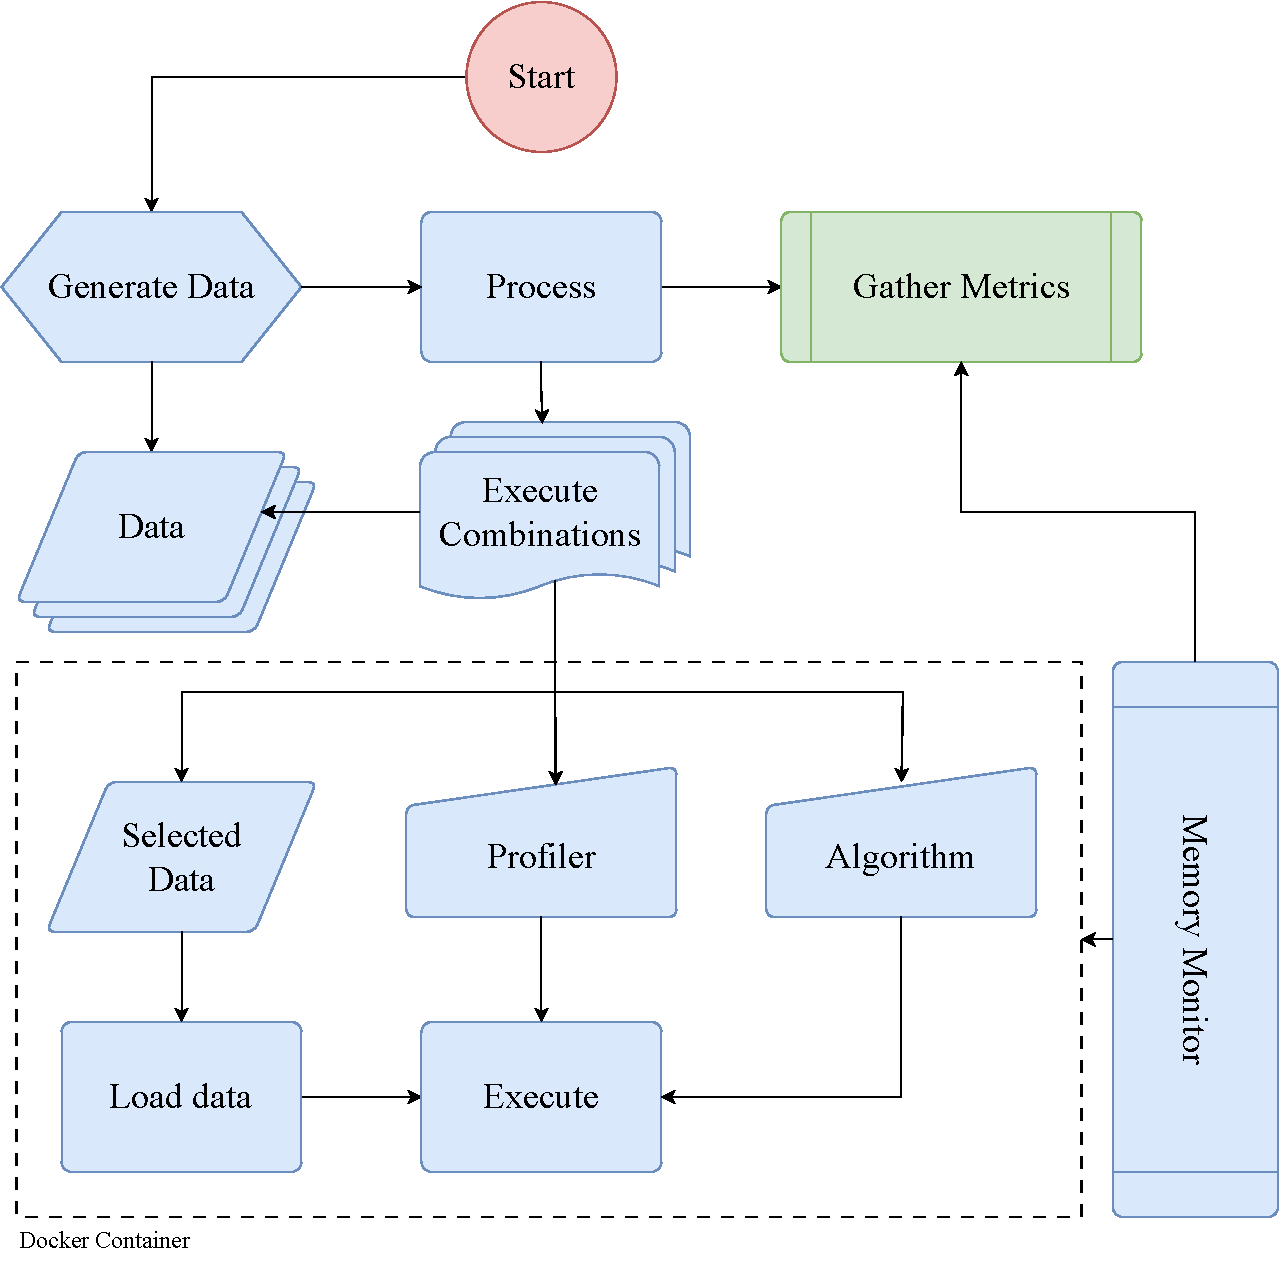
\includegraphics[width=0.8\textwidth]{./assets/images/04-experiment-flowchart}
    \caption{Flowchart illustrating the memory consumption experiment workflow.}
    \label{fig:mmc-experiment-workflow}
\end{figure}

\subsection{Evaluation Methodology}
\label{subsec:mmc-evaluation-methodology}

The evaluation of the experimental results was conducted using a multi-faceted approach that integrates statistical analysis and validation techniques.
This comprehensive methodology ensures that the analysis is both rigorous and reliable, providing meaningful insights into memory usage patterns, performance trends, and the computational efficiency of the algorithms.

The primary focus of the evaluation was to analyze three key aspects: memory efficiency, performance trends over time, and execution performance.
Each of these aspects offers a unique perspective on the algorithms’ behavior when analyzed with different profiling tools, enabling a comprehensive evaluation of the strengths and limitations of various memory measurement techniques.

In addition to the primary analysis, two validation techniques were employed to verify the accuracy and reliability of the collected data.
These validation methods ensure that the metrics accurately reflect the actual resource usage and performance characteristics of the experiments.

Table~\ref{tab:mmc-evaluation-criteria} summarizes the evaluation criteria and validation techniques used in this study.

\begin{table}[h]
    \centering
    \begin{tabular}{|l|p{6cm}|}
        \hline
        \textbf{Evaluation Criteria}     & \textbf{Description}                                                                                                                                                                                                                                 \\ \hline
        Memory Efficiency                & Evaluates \Mpeak across different algorithms, datasets, and profiling tools. By comparing these values, we can identify the differences between each memory measurement technique.                                                                   \\ \hline
        Performance Trends               & Analyzes \Mt to detect temporal consumption patterns, such as sudden spikes, gradual increases (indicative of memory leaks), and periods of stable usage.                                                                                            \\ \hline
        Execution Performance            & Correlates memory consumption metrics with \T to assess the trade-offs between memory usage and processing speed, providing insights into computational efficiency.                                                                                  \\ \hline
        Cross-Validation with Docker API & Verifies the internal memory usage data by comparing it with external monitoring results obtained through the Docker \ac{API}. This comparison helps ensure the consistency and reliability of the internal memory measurements.                     \\ \hline
        Memory Constraint Validation     & Re-executes experiments under constrained memory conditions, with limits set slightly below the previously recorded \Mpeak. This validation confirms whether the measured \Mpeak represents the minimum memory requirement for successful execution. \\ \hline
    \end{tabular}
    \caption{Evaluation criteria and validation techniques for the memory consumption experiments}
    \label{tab:mmc-evaluation-criteria}
\end{table}

The cross-validation with Docker \ac{API} data provided an external benchmark to verify the accuracy of the internal memory measurements.
By comparing the internal data with Docker's resource metrics, we ensured that the recorded memory usage reflected the actual resource consumption of the containerized environments.

Furthermore, the memory constraint validation served as a practical test to confirm the robustness of the peak memory usage measurements.
By limiting the available memory to slightly below the recorded \Mpeak, we observed whether the algorithm could still execute successfully.
Failure to complete the execution under these constrained conditions validated that the original \Mpeak measurement accurately represented the minimum memory required for the algorithm to run without errors.

This comprehensive evaluation framework ensures that the analysis of memory consumption and performance is both thorough and reliable, providing meaningful insights into the behavior of the algorithms under various resource constraints.

\subsection{Experiment Repository}
\label{subsec:mmc-experiment-repository}

You can find all the code, results, and experimental data used in the following repository: \DFTODO{Adicionar o link pro repositório}.


\section{Experimental Results}
\label{sec:mmc-results}

\DFTODO{Demonstrar resultados dos experimentos com viés (sem controlar o ambiente). Mostrando o impacto de execuções anteriores}
\DFTODO{Apresentar os resultados dos experimentos, mostrando o consumo de memória e o tempo de execução para cada algoritmo.}
\DFTODO{Destacar a validação feita para garantir a precisão das medições. Encontrando a questão da pressão de memória}
\DFTODO{Demonstrar o impacto ao aplicar pressão de memória}


\section{Conclusion}
\label{sec:mmc-conclusion}

\DFTODO{Concluir a respeito da necessidade de ambientes controlados para medir a memória}
\DFTODO{Concluir sobre as diferentes formas de medir a memória}
\DFTODO{Concluir sobre o garbage collector e a possibilidade de executar com pressão de memória}